% Options for packages loaded elsewhere
\PassOptionsToPackage{unicode}{hyperref}
\PassOptionsToPackage{hyphens}{url}
%
\documentclass[
]{article}
\usepackage{amsmath,amssymb}
\usepackage{iftex}
\ifPDFTeX
  \usepackage[T1]{fontenc}
  \usepackage[utf8]{inputenc}
  \usepackage{textcomp} % provide euro and other symbols
\else % if luatex or xetex
  \usepackage{unicode-math} % this also loads fontspec
  \defaultfontfeatures{Scale=MatchLowercase}
  \defaultfontfeatures[\rmfamily]{Ligatures=TeX,Scale=1}
\fi
\usepackage{lmodern}
\ifPDFTeX\else
  % xetex/luatex font selection
\fi
% Use upquote if available, for straight quotes in verbatim environments
\IfFileExists{upquote.sty}{\usepackage{upquote}}{}
\IfFileExists{microtype.sty}{% use microtype if available
  \usepackage[]{microtype}
  \UseMicrotypeSet[protrusion]{basicmath} % disable protrusion for tt fonts
}{}
\makeatletter
\@ifundefined{KOMAClassName}{% if non-KOMA class
  \IfFileExists{parskip.sty}{%
    \usepackage{parskip}
  }{% else
    \setlength{\parindent}{0pt}
    \setlength{\parskip}{6pt plus 2pt minus 1pt}}
}{% if KOMA class
  \KOMAoptions{parskip=half}}
\makeatother
\usepackage{xcolor}
\usepackage[margin=1in]{geometry}
\usepackage{color}
\usepackage{fancyvrb}
\newcommand{\VerbBar}{|}
\newcommand{\VERB}{\Verb[commandchars=\\\{\}]}
\DefineVerbatimEnvironment{Highlighting}{Verbatim}{commandchars=\\\{\}}
% Add ',fontsize=\small' for more characters per line
\usepackage{framed}
\definecolor{shadecolor}{RGB}{248,248,248}
\newenvironment{Shaded}{\begin{snugshade}}{\end{snugshade}}
\newcommand{\AlertTok}[1]{\textcolor[rgb]{0.94,0.16,0.16}{#1}}
\newcommand{\AnnotationTok}[1]{\textcolor[rgb]{0.56,0.35,0.01}{\textbf{\textit{#1}}}}
\newcommand{\AttributeTok}[1]{\textcolor[rgb]{0.13,0.29,0.53}{#1}}
\newcommand{\BaseNTok}[1]{\textcolor[rgb]{0.00,0.00,0.81}{#1}}
\newcommand{\BuiltInTok}[1]{#1}
\newcommand{\CharTok}[1]{\textcolor[rgb]{0.31,0.60,0.02}{#1}}
\newcommand{\CommentTok}[1]{\textcolor[rgb]{0.56,0.35,0.01}{\textit{#1}}}
\newcommand{\CommentVarTok}[1]{\textcolor[rgb]{0.56,0.35,0.01}{\textbf{\textit{#1}}}}
\newcommand{\ConstantTok}[1]{\textcolor[rgb]{0.56,0.35,0.01}{#1}}
\newcommand{\ControlFlowTok}[1]{\textcolor[rgb]{0.13,0.29,0.53}{\textbf{#1}}}
\newcommand{\DataTypeTok}[1]{\textcolor[rgb]{0.13,0.29,0.53}{#1}}
\newcommand{\DecValTok}[1]{\textcolor[rgb]{0.00,0.00,0.81}{#1}}
\newcommand{\DocumentationTok}[1]{\textcolor[rgb]{0.56,0.35,0.01}{\textbf{\textit{#1}}}}
\newcommand{\ErrorTok}[1]{\textcolor[rgb]{0.64,0.00,0.00}{\textbf{#1}}}
\newcommand{\ExtensionTok}[1]{#1}
\newcommand{\FloatTok}[1]{\textcolor[rgb]{0.00,0.00,0.81}{#1}}
\newcommand{\FunctionTok}[1]{\textcolor[rgb]{0.13,0.29,0.53}{\textbf{#1}}}
\newcommand{\ImportTok}[1]{#1}
\newcommand{\InformationTok}[1]{\textcolor[rgb]{0.56,0.35,0.01}{\textbf{\textit{#1}}}}
\newcommand{\KeywordTok}[1]{\textcolor[rgb]{0.13,0.29,0.53}{\textbf{#1}}}
\newcommand{\NormalTok}[1]{#1}
\newcommand{\OperatorTok}[1]{\textcolor[rgb]{0.81,0.36,0.00}{\textbf{#1}}}
\newcommand{\OtherTok}[1]{\textcolor[rgb]{0.56,0.35,0.01}{#1}}
\newcommand{\PreprocessorTok}[1]{\textcolor[rgb]{0.56,0.35,0.01}{\textit{#1}}}
\newcommand{\RegionMarkerTok}[1]{#1}
\newcommand{\SpecialCharTok}[1]{\textcolor[rgb]{0.81,0.36,0.00}{\textbf{#1}}}
\newcommand{\SpecialStringTok}[1]{\textcolor[rgb]{0.31,0.60,0.02}{#1}}
\newcommand{\StringTok}[1]{\textcolor[rgb]{0.31,0.60,0.02}{#1}}
\newcommand{\VariableTok}[1]{\textcolor[rgb]{0.00,0.00,0.00}{#1}}
\newcommand{\VerbatimStringTok}[1]{\textcolor[rgb]{0.31,0.60,0.02}{#1}}
\newcommand{\WarningTok}[1]{\textcolor[rgb]{0.56,0.35,0.01}{\textbf{\textit{#1}}}}
\usepackage{graphicx}
\makeatletter
\newsavebox\pandoc@box
\newcommand*\pandocbounded[1]{% scales image to fit in text height/width
  \sbox\pandoc@box{#1}%
  \Gscale@div\@tempa{\textheight}{\dimexpr\ht\pandoc@box+\dp\pandoc@box\relax}%
  \Gscale@div\@tempb{\linewidth}{\wd\pandoc@box}%
  \ifdim\@tempb\p@<\@tempa\p@\let\@tempa\@tempb\fi% select the smaller of both
  \ifdim\@tempa\p@<\p@\scalebox{\@tempa}{\usebox\pandoc@box}%
  \else\usebox{\pandoc@box}%
  \fi%
}
% Set default figure placement to htbp
\def\fps@figure{htbp}
\makeatother
\setlength{\emergencystretch}{3em} % prevent overfull lines
\providecommand{\tightlist}{%
  \setlength{\itemsep}{0pt}\setlength{\parskip}{0pt}}
\setcounter{secnumdepth}{-\maxdimen} % remove section numbering
\usepackage{ctex}
\usepackage{bookmark}
\IfFileExists{xurl.sty}{\usepackage{xurl}}{} % add URL line breaks if available
\urlstyle{same}
\hypersetup{
  pdftitle={homework3},
  pdfauthor={zza},
  hidelinks,
  pdfcreator={LaTeX via pandoc}}

\title{homework3}
\author{zza}
\date{2025-06-29}

\begin{document}
\maketitle

\subsection{1}\label{section}

\begin{Shaded}
\begin{Highlighting}[]
\CommentTok{\# 1. 读取数据并预处理}
\NormalTok{gmp }\OtherTok{\textless{}{-}} \FunctionTok{read.table}\NormalTok{(}\StringTok{"gmp.dat"}\NormalTok{, }\AttributeTok{header =} \ConstantTok{TRUE}\NormalTok{)  }
\NormalTok{gmp}\SpecialCharTok{$}\NormalTok{pop }\OtherTok{\textless{}{-}} \FunctionTok{round}\NormalTok{(gmp}\SpecialCharTok{$}\NormalTok{gmp }\SpecialCharTok{/}\NormalTok{ gmp}\SpecialCharTok{$}\NormalTok{pcgmp) }

\NormalTok{a1 }\OtherTok{\textless{}{-}} \FloatTok{0.1}  
\NormalTok{numerator1 }\OtherTok{\textless{}{-}} \FunctionTok{sum}\NormalTok{(gmp}\SpecialCharTok{$}\NormalTok{pcgmp }\SpecialCharTok{*}\NormalTok{ (gmp}\SpecialCharTok{$}\NormalTok{pop)}\SpecialCharTok{\^{}}\NormalTok{a1)}
\NormalTok{denominator1 }\OtherTok{\textless{}{-}} \FunctionTok{sum}\NormalTok{((gmp}\SpecialCharTok{$}\NormalTok{pop)}\SpecialCharTok{\^{}}\NormalTok{(}\DecValTok{2} \SpecialCharTok{*}\NormalTok{ a1))}
\NormalTok{y0\_1 }\OtherTok{\textless{}{-}}\NormalTok{ numerator1 }\SpecialCharTok{/}\NormalTok{ denominator1}

\NormalTok{a2 }\OtherTok{\textless{}{-}} \FloatTok{0.15}  
\NormalTok{numerator2 }\OtherTok{\textless{}{-}} \FunctionTok{sum}\NormalTok{(gmp}\SpecialCharTok{$}\NormalTok{pcgmp }\SpecialCharTok{*}\NormalTok{ (gmp}\SpecialCharTok{$}\NormalTok{pop)}\SpecialCharTok{\^{}}\NormalTok{a2)}
\NormalTok{denominator2 }\OtherTok{\textless{}{-}} \FunctionTok{sum}\NormalTok{((gmp}\SpecialCharTok{$}\NormalTok{pop)}\SpecialCharTok{\^{}}\NormalTok{(}\DecValTok{2} \SpecialCharTok{*}\NormalTok{ a2))}
\NormalTok{y0\_2 }\OtherTok{\textless{}{-}}\NormalTok{ numerator2 }\SpecialCharTok{/}\NormalTok{ denominator2}
\CommentTok{\# 定义幂律函数}
\NormalTok{power\_law }\OtherTok{\textless{}{-}} \ControlFlowTok{function}\NormalTok{(N, y0, a) \{}
\NormalTok{  y0 }\SpecialCharTok{*}\NormalTok{ N}\SpecialCharTok{\^{}}\NormalTok{a}
\NormalTok{\}}

\CommentTok{\# 绘制散点图(对数坐标)}
\FunctionTok{plot}\NormalTok{(gmp}\SpecialCharTok{$}\NormalTok{pop, gmp}\SpecialCharTok{$}\NormalTok{pcgmp,}
     \AttributeTok{log =} \StringTok{"xy"}\NormalTok{,}
     \AttributeTok{xlab =} \StringTok{"log(Pop)"}\NormalTok{, }
     \AttributeTok{ylab =} \StringTok{"l0g(PcGMP)"}\NormalTok{,}
     \AttributeTok{main =} \StringTok{"Per Capita GMP vs. Population"}\NormalTok{,}
     \AttributeTok{pch =} \DecValTok{20}\NormalTok{,    }\CommentTok{\# 点样式}
     \AttributeTok{col =} \StringTok{"blue"}\NormalTok{)}

\CommentTok{\# 添加3条曲线}
\FunctionTok{curve}\NormalTok{(}\FunctionTok{power\_law}\NormalTok{(x, }\AttributeTok{y0 =}\NormalTok{ y0\_1, }\AttributeTok{a =}\NormalTok{ a1),  }
      \AttributeTok{add =} \ConstantTok{TRUE}\NormalTok{, }\AttributeTok{col =} \StringTok{"red"}\NormalTok{, }\AttributeTok{lwd =} \DecValTok{2}\NormalTok{, }\AttributeTok{lty =} \DecValTok{1}\NormalTok{)}


\FunctionTok{curve}\NormalTok{(}\FunctionTok{power\_law}\NormalTok{(x, }\AttributeTok{y0 =}\NormalTok{ y0\_2, }\AttributeTok{a =}\NormalTok{ a2),  }\CommentTok{\# a = 0.10}
      \AttributeTok{add =} \ConstantTok{TRUE}\NormalTok{, }\AttributeTok{col =} \StringTok{"purple"}\NormalTok{, }\AttributeTok{lwd =} \DecValTok{2}\NormalTok{, }\AttributeTok{lty =} \DecValTok{2}\NormalTok{)}

\CommentTok{\# y0=6611, a=1/8}
\FunctionTok{curve}\NormalTok{(}\FunctionTok{power\_law}\NormalTok{(x, }\AttributeTok{y0 =} \DecValTok{6611}\NormalTok{, }\AttributeTok{a =} \DecValTok{1}\SpecialCharTok{/}\DecValTok{8}\NormalTok{),  }
      \AttributeTok{add =} \ConstantTok{TRUE}\NormalTok{, }\AttributeTok{col =} \StringTok{"green"}\NormalTok{, }\AttributeTok{lwd =} \DecValTok{2}\NormalTok{, }\AttributeTok{lty =} \DecValTok{3}\NormalTok{)}

\CommentTok{\# 图例}
\FunctionTok{legend}\NormalTok{(}\StringTok{"bottomleft"}\NormalTok{,               }
       \AttributeTok{legend =} \FunctionTok{c}\NormalTok{(                 }
         \FunctionTok{paste0}\NormalTok{(}\StringTok{"a = "}\NormalTok{, a1, }\StringTok{" (y0 = "}\NormalTok{, }\FunctionTok{round}\NormalTok{(y0\_1, }\DecValTok{1}\NormalTok{), }\StringTok{")"}\NormalTok{), }
         \FunctionTok{paste0}\NormalTok{(}\StringTok{"a = "}\NormalTok{, a2, }\StringTok{" (y0 = "}\NormalTok{, }\FunctionTok{round}\NormalTok{(y0\_2, }\DecValTok{1}\NormalTok{), }\StringTok{")"}\NormalTok{),}
         \StringTok{"a = 0.125 (y0 = 6611)"}  
\NormalTok{       ),}
       \AttributeTok{col =} \FunctionTok{c}\NormalTok{(}\StringTok{"red"}\NormalTok{, }\StringTok{"purple"}\NormalTok{, }\StringTok{"green"}\NormalTok{),  }
       \AttributeTok{lty =} \FunctionTok{c}\NormalTok{(}\DecValTok{1}\NormalTok{, }\DecValTok{2}\NormalTok{, }\DecValTok{3}\NormalTok{),                  }
       \AttributeTok{lwd =} \DecValTok{2}\NormalTok{,                  }
       \AttributeTok{title =} \StringTok{"Power Law Fits"}\NormalTok{) }
\end{Highlighting}
\end{Shaded}

\pandocbounded{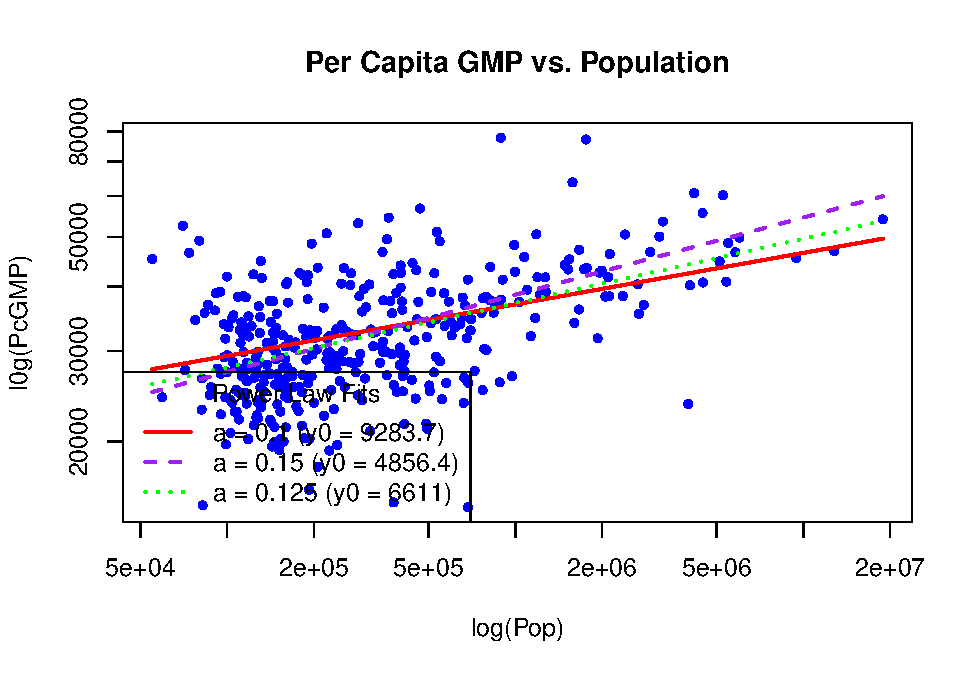
\includegraphics[keepaspectratio]{homework3_files/figure-latex/unnamed-chunk-1-1.pdf}}

\subsection{2}\label{section-1}

\begin{Shaded}
\begin{Highlighting}[]
\NormalTok{mse }\OtherTok{\textless{}{-}} \ControlFlowTok{function}\NormalTok{(params, }\AttributeTok{N =}\NormalTok{ gmp}\SpecialCharTok{$}\NormalTok{pop, }\AttributeTok{Y =}\NormalTok{ gmp}\SpecialCharTok{$}\NormalTok{pcgmp) \{}
\NormalTok{  y0 }\OtherTok{\textless{}{-}}\NormalTok{ params[}\DecValTok{1}\NormalTok{]}
\NormalTok{  a }\OtherTok{\textless{}{-}}\NormalTok{ params[}\DecValTok{2}\NormalTok{]}
  \ControlFlowTok{if}\NormalTok{ (a }\SpecialCharTok{\textless{}=} \DecValTok{0} \SpecialCharTok{||} \FunctionTok{any}\NormalTok{(N }\SpecialCharTok{\textless{}=} \DecValTok{0}\NormalTok{)) }\FunctionTok{return}\NormalTok{(}\FloatTok{1e10}\NormalTok{)  }
\NormalTok{  predictions }\OtherTok{\textless{}{-}}\NormalTok{ y0 }\SpecialCharTok{*}\NormalTok{ (N }\SpecialCharTok{\^{}}\NormalTok{ a)}
  \FunctionTok{mean}\NormalTok{((Y }\SpecialCharTok{{-}}\NormalTok{ predictions)}\SpecialCharTok{\^{}}\DecValTok{2}\NormalTok{) }
\NormalTok{\}}


\FunctionTok{mse}\NormalTok{(}\FunctionTok{c}\NormalTok{(}\DecValTok{6611}\NormalTok{, }\FloatTok{0.15}\NormalTok{))}
\end{Highlighting}
\end{Shaded}

\begin{verbatim}
## [1] 207057513
\end{verbatim}

\begin{Shaded}
\begin{Highlighting}[]
\FunctionTok{mse}\NormalTok{(}\FunctionTok{c}\NormalTok{(}\DecValTok{5000}\NormalTok{, }\FloatTok{0.10}\NormalTok{))}
\end{Highlighting}
\end{Shaded}

\begin{verbatim}
## [1] 298459914
\end{verbatim}

\subsection{3}\label{section-2}

\begin{Shaded}
\begin{Highlighting}[]
\CommentTok{\# 使用nlm()优化mse()}
\NormalTok{result1 }\OtherTok{\textless{}{-}} \FunctionTok{nlm}\NormalTok{(mse, }\FunctionTok{c}\NormalTok{(}\AttributeTok{y0 =} \DecValTok{4800}\NormalTok{, }\AttributeTok{a =} \FloatTok{0.1}\NormalTok{))}
\NormalTok{result2 }\OtherTok{\textless{}{-}}\FunctionTok{nlm}\NormalTok{(mse, }\FunctionTok{c}\NormalTok{(}\AttributeTok{y0 =} \DecValTok{6611}\NormalTok{, }\AttributeTok{a =} \DecValTok{1}\SpecialCharTok{/}\DecValTok{8}\NormalTok{))}
\NormalTok{result3 }\OtherTok{\textless{}{-}}\FunctionTok{nlm}\NormalTok{(mse, }\FunctionTok{c}\NormalTok{(}\AttributeTok{y0 =} \DecValTok{9000}\NormalTok{, }\AttributeTok{a =} \FloatTok{0.05}\NormalTok{))}

\CommentTok{\# 打印结果}
\FunctionTok{print}\NormalTok{(result1)}
\end{Highlighting}
\end{Shaded}

\begin{verbatim}
## $minimum
## [1] 62747987
## 
## $estimate
## [1] 4800.000001    0.150686
## 
## $gradient
## [1] -1244.134735    -2.503395
## 
## $code
## [1] 2
## 
## $iterations
## [1] 5
\end{verbatim}

\begin{Shaded}
\begin{Highlighting}[]
\FunctionTok{print}\NormalTok{(result2)}
\end{Highlighting}
\end{Shaded}

\begin{verbatim}
## $minimum
## [1] 61857060
## 
## $estimate
## [1] 6611.0000000    0.1263177
## 
## $gradient
## [1] 50.048639 -9.983778
## 
## $code
## [1] 2
## 
## $iterations
## [1] 3
\end{verbatim}

\begin{Shaded}
\begin{Highlighting}[]
\FunctionTok{print}\NormalTok{(result3)}
\end{Highlighting}
\end{Shaded}

\begin{verbatim}
## $minimum
## [1] 62861726
## 
## $estimate
## [1] 9000.0000004    0.1026275
## 
## $gradient
## [1] 678.014375   1.594424
## 
## $code
## [1] 2
## 
## $iterations
## [1] 6
\end{verbatim}

\textbf{结果解释}: - \texttt{minimum}:最小均方误差(MSE)。 -
\texttt{estimate}:最优参数(\(y_0\)和\(a\))。 -
初始值不同可能导致不同的收敛速度和结果。

\subsection{4}\label{section-3}

\begin{Shaded}
\begin{Highlighting}[]
\NormalTok{plm }\OtherTok{\textless{}{-}} \ControlFlowTok{function}\NormalTok{(y0\_init, a\_init, }\AttributeTok{N =}\NormalTok{ gmp}\SpecialCharTok{$}\NormalTok{pop, }\AttributeTok{Y =}\NormalTok{ gmp}\SpecialCharTok{$}\NormalTok{pcgmp) \{}
\NormalTok{  result }\OtherTok{\textless{}{-}} \FunctionTok{nlm}\NormalTok{(mse, }\FunctionTok{c}\NormalTok{(y0\_init, a\_init), }\AttributeTok{N =}\NormalTok{ N, }\AttributeTok{Y =}\NormalTok{ Y)}
  
  \FunctionTok{list}\NormalTok{(}
    \AttributeTok{y0 =}\NormalTok{ result}\SpecialCharTok{$}\NormalTok{estimate[}\DecValTok{1}\NormalTok{],}
    \AttributeTok{a =}\NormalTok{ result}\SpecialCharTok{$}\NormalTok{estimate[}\DecValTok{2}\NormalTok{],}
    \AttributeTok{mse =}\NormalTok{ result}\SpecialCharTok{$}\NormalTok{minimum}
\NormalTok{  )}
\NormalTok{\}}

\NormalTok{result1 }\OtherTok{\textless{}{-}} \FunctionTok{plm}\NormalTok{(}\AttributeTok{y0\_init =} \DecValTok{6611}\NormalTok{, }\AttributeTok{a\_init =} \FloatTok{0.15}\NormalTok{)}
\FunctionTok{print}\NormalTok{(result1)}
\end{Highlighting}
\end{Shaded}

\begin{verbatim}
## $y0
## [1] 6611
## 
## $a
## [1] 0.1263177
## 
## $mse
## [1] 61857060
\end{verbatim}

\begin{Shaded}
\begin{Highlighting}[]
\NormalTok{result2 }\OtherTok{\textless{}{-}} \FunctionTok{plm}\NormalTok{(}\AttributeTok{y0\_init =} \DecValTok{5000}\NormalTok{, }\AttributeTok{a\_init =} \FloatTok{0.10}\NormalTok{)}
\FunctionTok{print}\NormalTok{(result2)}
\end{Highlighting}
\end{Shaded}

\begin{verbatim}
## $y0
## [1] 5000
## 
## $a
## [1] 0.1475913
## 
## $mse
## [1] 62521484
\end{verbatim}

原因是非线性优化可能收敛到不同的局部最小值,初始值不同可能导致优化路径不同;

其中y从5000,a0从0.10开始的更小

\subsection{5}\label{section-4}

\subsubsection{a}\label{a}

\begin{verbatim}
## 均值: 32922.53
\end{verbatim}

\begin{verbatim}
## 经典标准误: 481.9195
\end{verbatim}

\subsubsection{b}\label{b}

\begin{Shaded}
\begin{Highlighting}[]
\NormalTok{jackknife\_mean }\OtherTok{\textless{}{-}} \ControlFlowTok{function}\NormalTok{(i, }\AttributeTok{data =}\NormalTok{ gmp}\SpecialCharTok{$}\NormalTok{pcgmp) \{}
  \FunctionTok{mean}\NormalTok{(data[}\SpecialCharTok{{-}}\NormalTok{i])  }\CommentTok{\# 排除第i个观测值}
\NormalTok{\}}
\end{Highlighting}
\end{Shaded}

\subsubsection{c}\label{c}

\begin{Shaded}
\begin{Highlighting}[]
\NormalTok{jackknifed.means }\OtherTok{\textless{}{-}} \FunctionTok{sapply}\NormalTok{(}\DecValTok{1}\SpecialCharTok{:}\FunctionTok{nrow}\NormalTok{(gmp), jackknife\_mean)}
\end{Highlighting}
\end{Shaded}

\subsubsection{d}\label{d}

\begin{Shaded}
\begin{Highlighting}[]
\CommentTok{\# 计算刀切方差和标准误}
\NormalTok{n }\OtherTok{\textless{}{-}} \FunctionTok{nrow}\NormalTok{(gmp)}
\NormalTok{jackknife\_var }\OtherTok{\textless{}{-}}\NormalTok{ ((n}\DecValTok{{-}1}\NormalTok{)}\SpecialCharTok{\^{}}\DecValTok{2}\SpecialCharTok{/}\NormalTok{n) }\SpecialCharTok{*} \FunctionTok{var}\NormalTok{(jackknifed.means)}
\NormalTok{jackknife\_sem }\OtherTok{\textless{}{-}} \FunctionTok{sqrt}\NormalTok{(jackknife\_var)}
\end{Highlighting}
\end{Shaded}

\begin{verbatim}
## 刀切标准误: 481.9195
\end{verbatim}

\begin{verbatim}
## 与传统标准误的比值: 1
\end{verbatim}

\subsection{6}\label{section-5}

\begin{Shaded}
\begin{Highlighting}[]
\NormalTok{plm.jackknife }\OtherTok{\textless{}{-}} \ControlFlowTok{function}\NormalTok{(y0\_init, a\_init, }\AttributeTok{N =}\NormalTok{ gmp}\SpecialCharTok{$}\NormalTok{pop, }\AttributeTok{Y =}\NormalTok{ gmp}\SpecialCharTok{$}\NormalTok{pcgmp) \{}
\NormalTok{  n }\OtherTok{\textless{}{-}} \FunctionTok{length}\NormalTok{(N)}
  
\NormalTok{  jack\_y0 }\OtherTok{\textless{}{-}} \FunctionTok{numeric}\NormalTok{(n)}
\NormalTok{  jack\_a }\OtherTok{\textless{}{-}} \FunctionTok{numeric}\NormalTok{(n)}

  \ControlFlowTok{for}\NormalTok{ (i }\ControlFlowTok{in} \DecValTok{1}\SpecialCharTok{:}\NormalTok{n) \{}

\NormalTok{    N\_sub }\OtherTok{\textless{}{-}}\NormalTok{ N[}\SpecialCharTok{{-}}\NormalTok{i]}
\NormalTok{    Y\_sub }\OtherTok{\textless{}{-}}\NormalTok{ Y[}\SpecialCharTok{{-}}\NormalTok{i]}
    
 
\NormalTok{    fit }\OtherTok{\textless{}{-}} \FunctionTok{plm}\NormalTok{(y0\_init, a\_init, N\_sub, Y\_sub)}
    
    
\NormalTok{    jack\_y0[i] }\OtherTok{\textless{}{-}}\NormalTok{ fit}\SpecialCharTok{$}\NormalTok{y0}
\NormalTok{    jack\_a[i] }\OtherTok{\textless{}{-}}\NormalTok{ fit}\SpecialCharTok{$}\NormalTok{a}
\NormalTok{  \}}
  
\NormalTok{  se\_y0 }\OtherTok{\textless{}{-}} \FunctionTok{sqrt}\NormalTok{(((n}\DecValTok{{-}1}\NormalTok{)}\SpecialCharTok{\^{}}\DecValTok{2}\SpecialCharTok{/}\NormalTok{n) }\SpecialCharTok{*} \FunctionTok{var}\NormalTok{(jack\_y0))}
\NormalTok{  se\_a }\OtherTok{\textless{}{-}} \FunctionTok{sqrt}\NormalTok{(((n}\DecValTok{{-}1}\NormalTok{)}\SpecialCharTok{\^{}}\DecValTok{2}\SpecialCharTok{/}\NormalTok{n) }\SpecialCharTok{*} \FunctionTok{var}\NormalTok{(jack\_a))}
  

  \FunctionTok{list}\NormalTok{(}\AttributeTok{se\_y0 =}\NormalTok{ se\_y0, }\AttributeTok{se\_a =}\NormalTok{ se\_a)}
\NormalTok{\}}

\CommentTok{\# 使用与问题4相同的初始值}
\NormalTok{jack\_result1 }\OtherTok{\textless{}{-}} \FunctionTok{plm.jackknife}\NormalTok{(}\AttributeTok{y0\_init =} \DecValTok{6611}\NormalTok{, }\AttributeTok{a\_init =} \FloatTok{0.15}\NormalTok{)}
\NormalTok{jack\_result2 }\OtherTok{\textless{}{-}} \FunctionTok{plm.jackknife}\NormalTok{(}\AttributeTok{y0\_init =} \DecValTok{5000}\NormalTok{, }\AttributeTok{a\_init =} \FloatTok{0.10}\NormalTok{)}

\FunctionTok{print}\NormalTok{(jack\_result1)}
\end{Highlighting}
\end{Shaded}

\begin{verbatim}
## $se_y0
## [1] 1.175826e-08
## 
## $se_a
## [1] 0.0009898304
\end{verbatim}

\begin{Shaded}
\begin{Highlighting}[]
\FunctionTok{print}\NormalTok{(jack\_result2)}
\end{Highlighting}
\end{Shaded}

\begin{verbatim}
## $se_y0
## [1] 2.033898e-08
## 
## $se_a
## [1] 0.0009979824
\end{verbatim}

\subsection{7}\label{section-6}

\begin{Shaded}
\begin{Highlighting}[]
\NormalTok{gmp2013 }\OtherTok{\textless{}{-}} \FunctionTok{read.table}\NormalTok{(}\StringTok{"gmp{-}2013.dat"}\NormalTok{, }\AttributeTok{header =} \ConstantTok{TRUE}\NormalTok{)}
\NormalTok{gmp2013}\SpecialCharTok{$}\NormalTok{pop }\OtherTok{\textless{}{-}} \FunctionTok{round}\NormalTok{(gmp2013}\SpecialCharTok{$}\NormalTok{gmp }\SpecialCharTok{/}\NormalTok{ gmp2013}\SpecialCharTok{$}\NormalTok{pcgmp)}



\CommentTok{\# 使用与2006年相同的初始值}
\NormalTok{fit2013 }\OtherTok{\textless{}{-}} \FunctionTok{plm}\NormalTok{(}\AttributeTok{y0\_init =} \DecValTok{5000}\NormalTok{, }\AttributeTok{a\_init =} \FloatTok{0.10}\NormalTok{, }
               \AttributeTok{N =}\NormalTok{ gmp2013}\SpecialCharTok{$}\NormalTok{pop, }\AttributeTok{Y =}\NormalTok{ gmp2013}\SpecialCharTok{$}\NormalTok{pcgmp)}

\CommentTok{\# 计算标准误}
\NormalTok{se2013 }\OtherTok{\textless{}{-}} \FunctionTok{plm.jackknife}\NormalTok{(}\AttributeTok{y0\_init =} \DecValTok{5000}\NormalTok{, }\AttributeTok{a\_init =} \FloatTok{0.10}\NormalTok{,}
                        \AttributeTok{N =}\NormalTok{ gmp2013}\SpecialCharTok{$}\NormalTok{pop, }\AttributeTok{Y =}\NormalTok{ gmp2013}\SpecialCharTok{$}\NormalTok{pcgmp)}


\FunctionTok{print}\NormalTok{(fit2013)}
\end{Highlighting}
\end{Shaded}

\begin{verbatim}
## $y0
## [1] 5000
## 
## $a
## [1] 0.164427
## 
## $mse
## [1] 139208731
\end{verbatim}

\begin{Shaded}
\begin{Highlighting}[]
\FunctionTok{print}\NormalTok{(se2013)}
\end{Highlighting}
\end{Shaded}

\begin{verbatim}
## $se_y0
## [1] 6.248473e-08
## 
## $se_a
## [1] 0.001122513
\end{verbatim}

\end{document}
